\section{Diseño del sistema: arquitectura base}
\label{sec:diseno}

% Diagramas de secuencia UML – arquitectura base
% Cada uno se define como un comando para incluirlo en su propia figura.
% Nota: en pgf-umlsd las etiquetas con paréntesis de \mess van entre llaves dobles.

\newcommand{\secuenciaConsultar}{%
{\footnotesize
\begin{sequencediagram}
    \newthread[morado!15]{c}{:Cliente}
    \newinst[1.6]{g}{:GestorTransacciones}
    \newinst[1.6]{r}{:ProcesadorRMC}
    \newinst[1.6]{p}{:ServicioPersistencia}
    \begin{call}{c}{consultarEventosMes(mes)}{g}{OK + filas}
        \begin{call}{g}{petición}{r}{respuesta}
            \begin{callself}{r}{validar AAAA-MM}{}
            \end{callself}
            \begin{call}{r}{listarFechasMes(mes)}{p}{OK + filas}
                \begin{callself}{p}{fechas del mes}{}
                \end{callself}
            \end{call}
        \end{call}
    \end{call}
\end{sequencediagram}}}

\newcommand{\secuenciaReservar}{%
{\footnotesize
\begin{sequencediagram}
    \newthread[morado!15]{c}{:Cliente}
    \newinst[1.6]{g}{:GestorTransacciones}
    \newinst[1.6]{r}{:ProcesadorRMC}
    \newinst[1.6]{p}{:ServicioPersistencia}
    \begin{call}{c}{reservar(idFecha, cupos)}{g}{OK idReserva}
        \begin{call}{g}{petición}{r}{respuesta}
            \begin{callself}{r}{validar datos}{}
            \end{callself}
            \begin{call}{r}{crearReserva}{p}{OK / ERROR}
                \begin{sdblock}{alt}{[idSolicitud ya procesado]}
                    \begin{callself}{p}{\shortstack[l]{devolver la\\respuesta guardada}}{}
                    \end{callself}
                \end{sdblock}
                \begin{callself}{p}{\shortstack[l]{validar estudiante,\\fecha y cupos}}{}
                \end{callself}
                \begin{callself}{p}{\shortstack[l]{aplicar todo o nada\\y guardar en bitácora}}{}
                \end{callself}
            \end{call}
        \end{call}
    \end{call}
\end{sequencediagram}}}

\newcommand{\secuenciaModificar}{%
{\footnotesize
\begin{sequencediagram}
    \newthread[morado!15]{c}{:Cliente}
    \newinst[1.6]{g}{:GestorTransacciones}
    \newinst[1.6]{r}{:ProcesadorRMC}
    \newinst[1.6]{p}{:ServicioPersistencia}
    \begin{call}{c}{modificarReserva}{g}{OK / ERROR}
        \begin{call}{g}{petición}{r}{respuesta}
            \begin{callself}{r}{validar datos}{}
            \end{callself}
            \begin{call}{r}{modificarReserva}{p}{OK / ERROR}
                \begin{callself}{p}{\shortstack[l]{verificar dueño, estado\\y cupos en la fecha destino}}{}
                \end{callself}
                \begin{callself}{p}{\shortstack[l]{liberar origen, ocupar destino,\\registrar transacción}}{}
                \end{callself}
            \end{call}
        \end{call}
    \end{call}
\end{sequencediagram}}}

\newcommand{\secuenciaCancelar}{%
{\footnotesize
\begin{sequencediagram}
    \newthread[morado!15]{c}{:Cliente}
    \newinst[1.8]{g}{:GestorTransacciones}
    \newinst[1.2]{r}{:ProcesadorRMC}
    \newinst[1.2]{x}{:ServicioCancelacion}
    \newinst[1.4]{p}{:ServicioPersistencia}
    \begin{call}{c}{cancelarReserva}{g}{EN\_PROCESO}
        \begin{call}{g}{petición}{r}{EN\_PROCESO}
            \begin{call}{r}{registrarCancelacion}{p}{OK}
                \begin{callself}{p}{\shortstack[l]{guardar solicitud\\PENDIENTE}}{}
                \end{callself}
            \end{call}
        \end{call}
        \mess{g}{{PUB aviso (idSolicitud)}}{x}
    \end{call}
    \begin{call}{x}{aplicarCancelacion}{p}{CONFIRMADA}
        \begin{callself}{p}{\shortstack[l]{liberar cupos, reserva\\CANCELADA, transacción}}{}
        \end{callself}
    \end{call}
    \mess{x}{{PUB notificación (CONFIRMADA)}}{c}
    \begin{sdblock}{loop}{[cada 2 s: barrido]}
        \begin{call}{x}{listarPendientes}{p}{PENDIENTES}
        \end{call}
    \end{sdblock}
\end{sequencediagram}}}


\subsection{Visión general}

La Figura~\ref{fig:arquitectura-basica} muestra la arquitectura básica que se
diseña en esta sección. En la \textbf{arquitectura base} hay exactamente una
instancia de cada componente.

\begin{figure}[htbp]
    \centering
    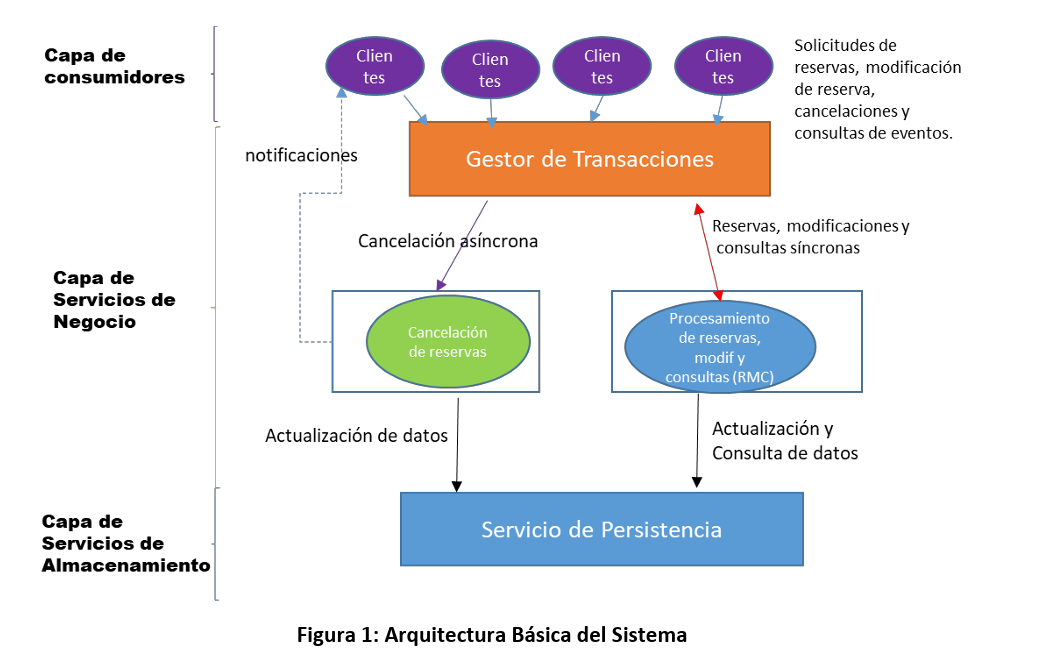
\includegraphics[width=0.92\textwidth]{figuras/arquitectura-basica.png}
    \caption{Arquitectura básica del sistema (Figura~1 del enunciado).}
    \label{fig:arquitectura-basica}
\end{figure}

\begin{itemize}
    \item \textbf{Clientes} (capa de consumidores): envían solicitudes de consulta,
          reserva, modificación y cancelación, y reciben notificaciones.
    \item \textbf{Gestor de Transacciones}: único punto de entrada de la capa de
          negocio. Las operaciones síncronas las envía al procesamiento RMC; las
          cancelaciones las publica para que se apliquen de forma asíncrona.
    \item \textbf{Procesamiento de reservas, modificaciones y consultas (RMC)}:
          valida y ejecuta las operaciones síncronas contra persistencia.
    \item \textbf{Cancelación de reservas}: aplica las cancelaciones y notifica al
          estudiante (línea punteada de la figura).
    \item \textbf{Servicio de Persistencia} (capa de almacenamiento): guarda los
          datos y aplica cada cambio de forma atómica.
\end{itemize}

\subsection{Comunicación entre componentes}

Toda la comunicación usa ZeroMQ (libzmq 4.3 con el enlace C++ cppzmq~\cite{cppzmq}).
La Tabla~\ref{tab:sockets} resume los sockets.

\begin{table}[H]
\centering
\caption{Sockets ZeroMQ de la arquitectura base.}
\label{tab:sockets}
\begin{tabularx}{\textwidth}{p{3.5cm}p{3.2cm}p{1.2cm}Y}
\toprule
Enlace & Sockets & Puerto & Uso \\
\midrule
Cliente $\rightarrow$ Gestor & \codigo{REQ} $\rightarrow$ \codigo{ROUTER} & 5555 &
Todas las solicitudes del estudiante; el cliente espera la respuesta. \\
Gestor $\leftrightarrow$ RMC & \codigo{ROUTER} $\leftrightarrow$ \codigo{DEALER} & 5556 &
El gestor reparte las peticiones entre los procesadores libres (patrón
\emph{load balancing broker}~\cite{zguide}). \\
Gestor $\rightarrow$ Cancelación & \codigo{PUB} $\rightarrow$ \codigo{SUB} & 5557 &
Aviso de cancelación aceptada (tema \codigo{cancelacion}). \\
Cancelación $\rightarrow$ Cliente & \codigo{PUB} $\rightarrow$ \codigo{SUB} & 5558 &
Notificación del resultado; cada cliente se suscribe al tema de su
\codigo{idEstudiante}. \\
RMC / Cancelación $\rightarrow$ Persistencia & \codigo{REQ} $\rightarrow$ \codigo{REP} & 5560 &
Consultas y cambios de datos. \\
\bottomrule
\end{tabularx}
\end{table}

\paragraph{Formato de los mensajes.} Cada mensaje es una trama de texto: la primera
línea es el tipo de operación y las siguientes son pares \codigo{clave=valor}; una
línea \codigo{--} abre una fila nueva para las respuestas con listas. Los errores
se responden con el tipo \codigo{ERROR} y los campos \codigo{codigo} y
\codigo{detalle}.

\begin{minipage}[t]{0.47\textwidth}
\begin{lstlisting}[title={Petición}]
reservar
idSolicitud=S-5f3a9c0d12e4b7a1
idEstudiante=EST-1
idFecha=F-1
cupos=2
\end{lstlisting}
\end{minipage}\hfill
\begin{minipage}[t]{0.47\textwidth}
\begin{lstlisting}[title={Respuesta}]
OK
idReserva=R-1
cupos=2
monto=0
disponibles=298
\end{lstlisting}
\end{minipage}

\subsection{Operaciones}

\begin{table}[H]
\centering
\caption{Operaciones del sistema.}
\label{tab:operaciones}
\small
\begin{tabularx}{\textwidth}{p{3.7cm}p{1.6cm}p{4.5cm}Y}
\toprule
Operación & Tipo & Operación en persistencia & Resultado \\
\midrule
\codigo{consultarEventosMes} & Síncrona & \codigo{listarFechasMes} &
Fechas del mes con evento, lugar, precio, límite, reservas y cupos disponibles. \\
\codigo{consultarReservas} & Síncrona & \codigo{listarReservasEstudiante} &
Reservas del estudiante y su estado. \\
\codigo{reservar} & Síncrona & \codigo{crearReserva} &
Reserva creada (\codigo{idReserva}, cupos, monto, disponibles). \\
\codigo{modificarReserva} & Síncrona & \codigo{modificarReserva} &
Nueva cantidad de cupos y/o fecha; diferencia de precio. \\
\codigo{cancelarReserva} & Asíncrona & \codigo{registrarCancelacion},
\codigo{aplicarCancelacion} & Respuesta inmediata \codigo{EN\_PROCESO}; luego
notificación \codigo{CONFIRMADA} o \codigo{FALLIDA}. \\
\bottomrule
\end{tabularx}
\end{table}

\paragraph{Reglas de negocio.} El límite de cupos de un evento es la capacidad de su
lugar (edificio o teatro registrado) o una capacidad definida a mano para lugares
externos. Las reservas de una fecha nunca superan ese límite; un estudiante tiene
como máximo una reserva activa por evento; las reservas y modificaciones se
aplican completas o no se aplican. Los códigos de error son:

\begin{itemize}\sloppy
    \item \textbf{de negocio:} \codigo{CUPOS\_INSUFICIENTES}, \codigo{RESERVA\_DUPLICADA},
          \codigo{FECHA\_NO\_EXISTE}, \codigo{ESTUDIANTE\_NO\_REGISTRADO},
          \codigo{RESERVA\_AJENA}, \codigo{CANCELACION\_PENDIENTE},
          \codigo{DATOS\_INVALIDOS};
    \item \textbf{técnicos:} \codigo{PERSISTENCIA\_NO\_DISPONIBLE},
          \codigo{SIN\_PROCESADORES}.
\end{itemize}

% =====================================================================
\subsection{Diagrama de despliegue}
\label{sec:despliegue}

La arquitectura base se despliega en las cuatro máquinas del laboratorio. Cada
máquina corre los ejecutables de una parte de la Figura~\ref{fig:arquitectura-basica};
los enlaces indican el protocolo y los puertos.

\begin{figure}[H]
    \centering
    \resizebox{\textwidth}{!}{% Diagrama de despliegue UML – arquitectura base
\begin{tikzpicture}[
    font=\small,
    artefacto/.style={draw, fill=white, rounded corners=1pt, minimum width=4.8cm,
                      minimum height=1.05cm, align=center, inner sep=3pt},
    archivo/.style={artefacto, fill=gris!8},
    titulo/.style={align=center, inner sep=2pt},
    maquina/.style={draw, thick, fill=azulclaro, inner sep=0.3cm},
    enlace/.style={thick, draw=azul},
    etiqueta/.style={font=\scriptsize, fill=white, align=center, inner sep=1.5pt},
]
    % Dibuja el efecto 3D de un nodo UML
    \newcommand{\cubo}[1]{%
        \draw[thick, fill=azulclaro!60] (#1.north west) -- ++(0.3,0.3) -- ($(#1.north east)+(0.3,0.3)$)
            -- ($(#1.south east)+(0.3,0.3)$) -- (#1.south east) -- (#1.north east) -- cycle;
        \draw[thick] (#1.north east) -- ++(0.3,0.3);}

    % ---------------- Máquina 1: clientes
    \node[titulo] (t1) at (0,0) {\guillemotleft device\guillemotright\\\textbf{Máquina 1 – Clientes}};
    \node[artefacto, below=0.2cm of t1] (cli1) {\guillemotleft artifact\guillemotright\\\codigo{bin/cliente} (estudiante 1)};
    \node[artefacto, below=0.25cm of cli1] (cli2) {\guillemotleft artifact\guillemotright\\\codigo{bin/cliente} (estudiante 2)};
    \node[below=0.02cm of cli2] (clin) {\Large $\vdots$};
    \node[artefacto, below=0.02cm of clin] (cli3) {\guillemotleft artifact\guillemotright\\\codigo{bin/cliente} (estudiante N)};

    % ---------------- Máquina 2: gestor
    \node[titulo] (t2) at (9.5,0) {\guillemotleft device\guillemotright\\\textbf{Máquina 2 – Gestor}};
    \node[artefacto, below=0.2cm of t2] (ges) {\guillemotleft artifact\guillemotright\\\codigo{bin/gestor-transacciones}};

    % ---------------- Máquina 3: procesos de negocio
    \node[titulo] (t3) at (9.5,-4.4) {\guillemotleft device\guillemotright\\\textbf{Máquina 3 – Negocio}};
    \node[artefacto, below=0.2cm of t3] (rmc) {\guillemotleft artifact\guillemotright\\\codigo{bin/procesador-rmc}};
    \node[artefacto, below=0.25cm of rmc] (can) {\guillemotleft artifact\guillemotright\\\codigo{bin/cancelacion-reservas}};

    % ---------------- Máquina 4: persistencia
    \node[titulo] (t4) at (9.5,-10.2) {\guillemotleft device\guillemotright\\\textbf{Máquina 4 – Almacenamiento}};
    \node[artefacto, below=0.2cm of t4] (per) {\guillemotleft artifact\guillemotright\\\codigo{bin/persistencia}};
    \node[archivo, below=0.25cm of per] (bit) {\guillemotleft file\guillemotright\\\codigo{datos/bitacora.txt}};

    \begin{scope}[on background layer]
        \node[maquina, fit=(t1)(cli1)(cli3)] (m1) {};
        \node[maquina, fit=(t2)(ges)] (m2) {};
        \node[maquina, fit=(t3)(rmc)(can)] (m3) {};
        \node[maquina, fit=(t4)(per)(bit)] (m4) {};
        \cubo{m1} \cubo{m2} \cubo{m3} \cubo{m4}
    \end{scope}

    % ---------------- Enlaces de red
    \draw[enlace] (m2.west) -- node[etiqueta, above=3pt] {\guillemotleft TCP / ZeroMQ\guillemotright\\REQ $\rightarrow$ ROUTER :5555} (m2.west -| m1.east);
    \draw[enlace] (m2.south) -- node[etiqueta, right=3pt] {\guillemotleft TCP / ZeroMQ\guillemotright\\ROUTER :5556 $\leftrightarrow$ DEALER\\PUB :5557 $\rightarrow$ SUB} (m3.north);
    \draw[enlace] (m3.south) -- node[etiqueta, right=3pt] {\guillemotleft TCP / ZeroMQ\guillemotright\\REQ $\rightarrow$ REP :5560} (m4.north);
    \draw[enlace, dashed] (m3.west) -| node[etiqueta, pos=0.3, below=3pt] {\guillemotleft TCP / ZeroMQ\guillemotright\\notificaciones\\PUB :5558 $\rightarrow$ SUB} (m1.south);
\end{tikzpicture}
}
    \caption{Diagrama de despliegue de la arquitectura base.}
    \label{fig:despliegue}
\end{figure}

% =====================================================================
\subsection{Diagrama de componentes}

Cada componente ofrece y requiere interfaces ZeroMQ. El símbolo de bola indica la
interfaz que un componente provee y el de semicírculo la que otro requiere.

\begin{figure}[H]
    \centering
    \resizebox{!}{0.62\textheight}{% Diagrama de componentes UML – arquitectura base
\begin{tikzpicture}[
    font=\small,
    componente/.style={draw, thick, fill=white, minimum width=4.4cm, minimum height=1.5cm,
                       align=center, inner sep=4pt},
    capa/.style={draw=gris, dashed, rounded corners=4pt, inner sep=0.45cm},
    nombrecapa/.style={font=\footnotesize\bfseries, text=gris, anchor=north west},
    interfaz/.style={font=\scriptsize, align=center, fill=white, inner sep=1pt},
]
    % Icono de componente UML en la esquina superior derecha del nodo
    \newcommand{\icono}[1]{%
        \draw[fill=white] ($(#1.north east)+(-0.55,-0.18)$) rectangle ++(0.36,-0.42);
        \draw[fill=white] ($(#1.north east)+(-0.63,-0.27)$) rectangle ++(0.16,-0.08);
        \draw[fill=white] ($(#1.north east)+(-0.63,-0.44)$) rectangle ++(0.16,-0.08);}
    % Conector de ensamblaje vertical: #1 requiere (arriba), #2 provee (abajo), #3 punto, #4 nombre
    \newcommand{\ensambleV}[4]{%
        \draw[thick] (#2) -- (#3);
        \draw[thick, fill=white] (#3) circle (0.14);
        \draw[thick] (#1) -- ($(#3)+(0,0.26)$);
        \draw[thick] ($(#3)+(0.26,0)$) arc (0:180:0.26);
        \node[interfaz, right=0.32cm of #3] {#4};}

    % ---------------- Consumidores
    \node[componente, fill=morado!12] (cli) at (0,0)
        {\guillemotleft component\guillemotright\\\textbf{Cliente}\\\scriptsize \codigo{Cliente}, \codigo{ConsolaCliente}};

    % ---------------- Negocio
    \node[componente, fill=naranja!20] (ges) at (0,-3.6)
        {\guillemotleft component\guillemotright\\\textbf{Gestor de Transacciones}\\\scriptsize \codigo{GestorTransacciones}};
    \node[componente, fill=azul!15] (rmc) at (-3.4,-7.4)
        {\guillemotleft component\guillemotright\\\textbf{Procesamiento RMC}\\\scriptsize \codigo{ProcesadorRMC}};
    \node[componente, fill=verde!25] (can) at (3.4,-7.4)
        {\guillemotleft component\guillemotright\\\textbf{Cancelación de reservas}\\\scriptsize \codigo{ServicioCancelacion}};

    % ---------------- Almacenamiento
    \node[componente, fill=azul!25, minimum width=6.5cm] (per) at (0,-11.4)
        {\guillemotleft component\guillemotright\\\textbf{Servicio de Persistencia}\\\scriptsize \codigo{ServicioPersistencia}, \codigo{BaseDatos}, \codigo{Almacenamiento}};

    \foreach \c in {cli, ges, rmc, can, per} {\icono{\c}}

    % ---------------- Interfaces
    % Cliente requiere ISolicitudes (provista por el gestor)
    \coordinate (i1) at (0,-1.85);
    \ensambleV{cli.south}{ges.north}{i1}{\codigo{ISolicitudes}\\ROUTER :5555};

    % Gestor requiere IProcesamiento (provista por los procesadores RMC)
    \coordinate (i2) at (-3.4,-5.6);
    \draw[thick] (rmc.north) -- (i2);
    \draw[thick, fill=white] (i2) circle (0.14);
    \draw[thick] (ges.south west) ++(0.8,0) |- ($(i2)+(0,0.9)$) -- ($(i2)+(0,0.26)$);
    \draw[thick] ($(i2)+(0.26,0)$) arc (0:180:0.26);
    \node[interfaz, left=0.32cm of i2] {\codigo{IProcesamiento}\\ROUTER :5556 / DEALER};

    % Cancelación requiere IAvisosCancelacion (provista por el gestor, PUB)
    \coordinate (i3) at (3.4,-5.6);
    \draw[thick] (ges.south east) ++(-0.8,0) |- ($(i3)+(0,0.9)$) -- (i3);
    \draw[thick, fill=white] (i3) circle (0.14);
    \draw[thick] (can.north) -- ($(i3)+(0,-0.26)$);
    \draw[thick] ($(i3)+(-0.26,0)$) arc (180:360:0.26);
    \node[interfaz, right=0.32cm of i3] {\codigo{IAvisosCancelacion}\\PUB :5557 / SUB};

    % Cliente requiere INotificaciones (provista por cancelación, PUB)
    \coordinate (i4) at (6.6,0);
    \draw[thick, dashed] (can.east) -| (i4);
    \draw[thick, fill=white] (i4) circle (0.14);
    \draw[thick, dashed] (cli.east) -- ($(i4)+(-0.26,0)$);
    \draw[thick] ($(i4)+(0,0.26)$) arc (90:270:0.26);
    \node[interfaz, above=0.3cm of i4] {\codigo{INotificaciones}\\PUB :5558 / SUB};

    % RMC y cancelación requieren IPersistencia
    \coordinate (i5) at (0,-9.6);
    \draw[thick] (per.north) -- (i5);
    \draw[thick, fill=white] (i5) circle (0.14);
    \draw[thick] (rmc.south) |- ($(i5)+(-0.6,0.5)$) -- ($(i5)+(0,0.5)$) -- ($(i5)+(0,0.26)$);
    \draw[thick] (can.south) |- ($(i5)+(0.6,0.5)$) -- ($(i5)+(0,0.5)$);
    \draw[thick] ($(i5)+(0.26,0)$) arc (0:180:0.26);
    \node[interfaz, right=0.32cm of i5] {\codigo{IPersistencia}\\REP :5560};

    % ---------------- Capas
    \begin{scope}[on background layer]
        \node[capa, fit=(cli)] (c1) {};
        \node[nombrecapa] at (c1.north west) {Capa de consumidores};
        \node[capa, fit=(ges)(rmc)(can)] (c2) {};
        \node[nombrecapa] at (c2.north west) {Capa de Servicios de Negocio};
        \node[capa, fit=(per)] (c3) {};
        \node[nombrecapa] at (c3.north west) {Capa de Servicios de Almacenamiento};
    \end{scope}
\end{tikzpicture}
}
    \caption{Diagrama de componentes de la arquitectura base.}
    \label{fig:componentes}
\end{figure}

% =====================================================================
\subsection{Diagramas de clases}

El sistema está escrito en C++17 orientado a objetos. La
Figura~\ref{fig:clases-servicios} muestra las clases de los procesos y la
Figura~\ref{fig:clases-dominio} el modelo de dominio que guarda persistencia.
Las decisiones de diseño orientado a objetos más importantes son:

\begin{itemize}
    \item \textbf{Herencia y método plantilla:} \codigo{Servicio::ejecutar()} define el
          ciclo de vida común (señales, \codigo{inicializar}, \codigo{iterar},
          \codigo{finalizar}) y cada proceso implementa sus pasos.
    \item \textbf{Polimorfismo:} \codigo{Lugar} es abstracta; \codigo{LugarUniversidad}
          y \codigo{LugarExterno} calculan la capacidad de forma distinta y
          \codigo{Evento} no necesita saber cuál tiene.
    \item \textbf{Interfaz intercambiable:} \codigo{Almacenamiento} separa la lógica de
          datos de cómo se guardan; hoy es un archivo de bitácora y luego podrá ser
          PostgreSQL sin cambiar \codigo{BaseDatos}.
    \item \textbf{Encapsulamiento:} las reglas de cupos viven en \codigo{FechaEvento}
          y las de estado en \codigo{Reserva} y \codigo{SolicitudCancelacion}.
    \item \textbf{Reutilización:} \codigo{ClienteConfiable} implementa el patrón
          \emph{Lazy Pirate} una sola vez y lo usan el cliente y los procesos de negocio.
\end{itemize}

\begin{sidewaysfigure}
    \centering
    \resizebox{\linewidth}{!}{% Diagrama de clases UML – procesos, comunicación y almacenamiento
\begin{tikzpicture}[font=\footnotesize]
    % ---------------- Clase base de los procesos servidores
    \begin{abstractclass}[text width=6.2cm]{Servicio}{11.2,0}
        \attribute{- nombre : string}
        \attribute{- contexto : zmq::context\_t}
        \operation{+ ejecutar() : int}
        \operation[0]{\# inicializar() : void}
        \operation[0]{\# iterar() : void}
        \operation{\# finalizar() : void}
    \end{abstractclass}

    % ---------------- Procesos
    \begin{class}[text width=6.6cm]{GestorTransacciones}{0,-5.2}
        \inherit{Servicio}
        \attribute{- frontend : socket ROUTER}
        \attribute{- backend : socket ROUTER}
        \attribute{- publicador : socket PUB}
        \attribute{- procesadoresLibres : deque<string>}
        \attribute{- ultimoContacto : map<string,long>}
        \operation{- atenderCliente() : void}
        \operation{- atenderProcesador() : void}
        \operation{- enviarAProcesador(...) : bool}
        \operation{- publicarCancelacion(Mensaje) : void}
    \end{class}

    \begin{class}[text width=6.6cm]{ProcesadorRMC}{7.4,-5.2}
        \inherit{Servicio}
        \attribute{- gestor : socket DEALER}
        \operation{- procesar(Mensaje) : Mensaje}
        \operation{- consultarEventosMes(Mensaje) : Mensaje}
        \operation{- reservar(Mensaje) : Mensaje}
        \operation{- modificarReserva(Mensaje) : Mensaje}
        \operation{- cancelarReserva(Mensaje) : Mensaje}
        \operation{- enviarLatido() : void}
    \end{class}

    \begin{class}[text width=5.8cm]{ServicioCancelacion}{14.6,-5.2}
        \inherit{Servicio}
        \attribute{- avisos : socket SUB}
        \attribute{- notificaciones : socket PUB}
        \operation{- procesar(idSolicitud) : void}
        \operation{- barrer() : void}
        \operation{- notificar(Mensaje) : void}
    \end{class}

    \begin{class}[text width=5.6cm]{ServicioPersistencia}{21.4,-5.2}
        \inherit{Servicio}
        \attribute{- socket : socket REP}
        \operation{- atender(Mensaje) : Mensaje}
        \operation{- aplicar(Mensaje) : Mensaje}
    \end{class}

    % ---------------- Apoyo
    \begin{class}[text width=6.8cm]{ClienteConfiable}{10.9,-12.2}
        \attribute{- endpoint : string}
        \attribute{- timeout : milliseconds}
        \attribute{- intentos : int}
        \attribute{- socket : socket REQ}
        \operation{+ solicitar(Mensaje) : optional<Mensaje>}
    \end{class}

    \begin{class}[text width=6.6cm]{BaseDatos}{18.6,-12.2}
        \operation{+ listarFechasMes(Mensaje) : Mensaje}
        \operation{+ listarReservasEstudiante(Mensaje) : Mensaje}
        \operation{+ crearReserva(Mensaje) : Mensaje}
        \operation{+ modificarReserva(Mensaje) : Mensaje}
        \operation{+ registrarCancelacion(Mensaje) : Mensaje}
        \operation{+ aplicarCancelacion(Mensaje) : Mensaje}
        \operation{+ respuestaPrevia(clave) : Mensaje*}
    \end{class}

    \begin{interface}[text width=5.2cm]{Almacenamiento}{25.4,-12.2}
        \operation[0]{+ cargar() : vector<Mensaje>}
        \operation[0]{+ registrar(Mensaje) : void}
    \end{interface}

    \begin{class}[text width=5.2cm]{AlmacenamientoArchivo}{25.4,-16.2}
        \implement{Almacenamiento}
        \attribute{- ruta : string}
    \end{class}

    \begin{class}[text width=6.4cm]{Mensaje}{2.4,-12.2}
        \attribute{- tipo : string}
        \attribute{- campos : map<string,string>}
        \attribute{- filas : vector<Fila>}
        \operation{+ poner(clave, valor) : Mensaje\&}
        \operation{+ texto(clave) : string}
        \operation{+ serializar() : string}
        \operation{+ deserializar(string) : Mensaje}
    \end{class}

    % ---------------- Consumidores
    \begin{class}[text width=6.6cm]{Cliente}{2.4,-18.0}
        \attribute{- idEstudiante : string}
        \operation{+ consultarEventosMes(mes) : Mensaje}
        \operation{+ reservar(idFecha, cupos) : Mensaje}
        \operation{+ modificarReserva(...) : Mensaje}
        \operation{+ cancelarReserva(idReserva) : Mensaje}
        \operation{+ notificacionesPendientes() : vector}
    \end{class}

    \begin{class}[text width=4.4cm]{ConsolaCliente}{10.9,-18.8}
        \operation{+ ejecutar() : int}
    \end{class}

    % ---------------- Relaciones
    \composition{ProcesadorRMC}{}{}{ClienteConfiable}
    \composition{ServicioCancelacion}{}{}{ClienteConfiable}
    \composition{ServicioPersistencia}{}{}{BaseDatos}
    \aggregation{ServicioPersistencia}{}{}{Almacenamiento}
    \composition{Cliente}{}{}{ClienteConfiable}
    \unidirectionalAssociation{ConsolaCliente}{usa}{1}{Cliente}
    \draw[umlcd style dashed line, ->] (GestorTransacciones) -- node[left, font=\scriptsize] {\guillemotleft use\guillemotright} (Mensaje);
\end{tikzpicture}
}
    \caption{Diagrama de clases de los procesos y la comunicación.}
    \label{fig:clases-servicios}
\end{sidewaysfigure}

\begin{sidewaysfigure}
    \centering
    \resizebox{\linewidth}{!}{% Diagrama de clases UML – modelo de dominio (capa de almacenamiento)
\begin{tikzpicture}[font=\footnotesize]
    \begin{abstractclass}[text width=4.4cm]{Lugar}{0,0}
        \operation[0]{+ capacidad() : int}
        \operation[0]{+ descripcion() : string}
    \end{abstractclass}

    \begin{class}[text width=4.4cm]{LugarUniversidad}{-2.6,-4.6}
        \inherit{Lugar}
        \attribute{- id : string}
        \attribute{- nombre : string}
        \attribute{- tipo : EDIFICIO | TEATRO}
        \attribute{- capacidad : int}
    \end{class}

    \begin{class}[text width=4.0cm]{LugarExterno}{2.6,-4.6}
        \inherit{Lugar}
        \attribute{- direccion : string}
        \attribute{- capacidad : int}
    \end{class}

    \begin{class}[text width=4.6cm]{Evento}{8.4,0}
        \attribute{- id : string}
        \attribute{- nombre : string}
        \attribute{- precio : long}
        \operation{+ limite() : int}
    \end{class}

    \begin{class}[text width=5.4cm]{FechaEvento}{8.4,-5.6}
        \attribute{- id : string}
        \attribute{- fecha : string}
        \attribute{- reservas : int}
        \operation{+ mes() : string}
        \operation{+ hayCupo(cupos, limite) : bool}
        \operation{+ ocupar(cupos) : void}
        \operation{+ liberar(cupos) : void}
    \end{class}

    \begin{class}[text width=5.0cm]{Estudiante}{14.8,0}
        \attribute{- codigo : string}
        \attribute{- nombre : string}
        \attribute{- tipoDocumento : string}
        \attribute{- numeroDocumento : string}
        \attribute{- carrera : string}
        \attribute{- departamento : string}
        \attribute{- semestre : int}
        \attribute{- correo : string}
        \attribute{- telefono : string}
    \end{class}

    \begin{class}[text width=5.4cm]{Reserva}{14.8,-7.0}
        \attribute{- id : string}
        \attribute{- cupos : int}
        \attribute{- estado : ACTIVA | CANCELADA}
        \operation{+ cambiar(cupos, idFecha) : void}
        \operation{+ cancelar() : void}
    \end{class}

    \begin{class}[text width=6.4cm]{Transaccion}{22.4,-7.0}
        \attribute{- id : string}
        \attribute{- idSolicitud : string}
        \attribute{- tipo : RESERVA | MODIFICACION | CANCELACION}
        \attribute{- cupos : int}
        \attribute{- monto : long}
        \attribute{- instante : long}
    \end{class}

    \begin{class}[text width=6.4cm]{SolicitudCancelacion}{22.4,0}
        \attribute{- idSolicitud : string}
        \attribute{- estado : PENDIENTE | CONFIRMADA | FALLIDA}
        \attribute{- creada : long}
        \operation{+ confirmar() : void}
        \operation{+ fallar(detalle) : void}
    \end{class}

    \unidirectionalAssociation{Evento}{se realiza en}{1}{Lugar}
    \composition{Evento}{fechas}{1..*}{FechaEvento}
    \association{Estudiante}{}{1}{Reserva}{reservas}{0..*}
    \unidirectionalAssociation{Reserva}{fecha}{1}{FechaEvento}
    \association{Reserva}{}{1}{Transaccion}{historial}{1..*}
    \unidirectionalAssociation{SolicitudCancelacion}{cancela}{1}{Reserva}
\end{tikzpicture}
}
    \caption{Diagrama de clases del modelo de dominio.}
    \label{fig:clases-dominio}
\end{sidewaysfigure}
\clearpage

% =====================================================================
\subsection{Diagramas de secuencia}

\paragraph{Consultar los eventos de un mes.} El gestor entrega la petición a un
procesador RMC libre, que valida el mes y pide a persistencia las fechas.

\begin{figure}[H]
    \centering
    \secuenciaConsultar
    \caption{Secuencia: consultar los eventos de un mes.}
\end{figure}

\paragraph{Reservar.} Persistencia revisa primero si el \codigo{idSolicitud} ya se
procesó (reintento); si no, valida todo y aplica el cambio de forma atómica.

\begin{figure}[H]
    \centering
    \resizebox{\textwidth}{!}{\secuenciaReservar}
    \caption{Secuencia: reservar cupos.}
\end{figure}

\paragraph{Modificar una reserva.} Igual que la reserva, pero libera los cupos de la
fecha original y ocupa los de la fecha destino en una sola operación.

\begin{figure}[H]
    \centering
    \resizebox{\textwidth}{!}{\secuenciaModificar}
    \caption{Secuencia: modificar una reserva.}
\end{figure}

\paragraph{Cancelar una reserva (asíncrona).} La solicitud se guarda como
\codigo{PENDIENTE} \emph{antes} de responder; así, aunque el aviso PUB/SUB se
pierda, el barrido periódico la encuentra y la aplica. El estudiante recibe de
inmediato \codigo{EN\_PROCESO} y después la notificación con el resultado.

\begin{figure}[H]
    \centering
    \resizebox{\textwidth}{!}{\secuenciaCancelar}
    \caption{Secuencia: cancelar una reserva (asíncrona).}
\end{figure}
